\documentclass[a4paper]{scrartcl}

% font/encoding packages
\usepackage[utf8]{inputenc}
\usepackage[T1]{fontenc}
\usepackage{lmodern}
\usepackage[ngerman]{babel}
\usepackage[ngerman=ngerman-x-latest]{hyphsubst}

\usepackage{amsmath, amssymb, amsfonts, amsthm}
\usepackage{array}
\usepackage{stmaryrd}
\usepackage{marvosym}
\allowdisplaybreaks
\usepackage[output-decimal-marker={,}]{siunitx}
\usepackage[shortlabels]{enumitem}
\usepackage[section]{placeins}
\usepackage{float}
\usepackage{units}
\usepackage{listings}
\usepackage{pgfplots}
\pgfplotsset{compat=1.12}
\usepackage{tikz}
\usetikzlibrary{arrows,automata}

\usepackage{xcolor}
\definecolor{light-gray}{HTML}{cccccc}


\newtheorem*{behaupt}{Behauptung}
\newcommand{\gdw}{\Leftrightarrow}
\newcommand{\dif}{\ \mathrm{d}}
\newcommand{\N}{\mathbb{N}}
\newcommand{\prob}{\mathbb{P}}
\newcommand{\cov}{\operatorname{Cov}}
\newcommand{\e}{\mathbb{E}}
\newcommand{\var}{\operatorname{Var}}
\newcommand{\corr}{\operatorname{Corr}}

\usepackage{fancyhdr}
\pagestyle{fancy}

\lstset{%
    frame=single,
    numbers=left,
    keepspaces,
    language=R,
    title=Listing: \lstname,
}

\def \blattnr {12}

\lhead{Stochastik 2 - Blatt {\blattnr}}
\rhead{Florian Abt, Lennart Braun, Sascha Schulz}
\cfoot{\thepage}


\title{Stochastik 2 für Informatiker}
\subtitle{Blatt {\blattnr} Hausaufgaben}
\author{
    Florian Abt (6524404), \\
    Lennart Braun (6523742), \\
    Sascha Schulz (6434677)
}
\date{zum 19. Januar 2016}
\usepackage{pdfpages} 

\begin{document}
\maketitle

\begin{enumerate}[label=\bfseries \blattnr.\arabic*]
    \item %.1
        % Im Fall von k=0.5 scheint die Breite der Konfidenzintervalle bei
        % steigendem n und konstantem Konfidenzniveau monoton zu fallen.
        % 
        % Bei k=1.5 und k=2.5 ist diese Monotonie nur bedingt zu beobachten, es
        % kommt zu Sprungstellen, in denen einzelne (seltene) extreme Werte
        % dazu führen, dass das Konfidenzintervalle sprungartig wieder sehr
        % viel breiter wird.
        %
        % Habe vor allem beobachtet, dass die Ausreißer bei k=0.5 wesentlich
        % mehr Einfluss auf die Breite des Konfidenzintervals haben.


       Bei $k=\num{0,5}$ nehmen die Ausreißer besonders hohe Werte an. Diese
       sorgen dafür, dass die Konfidenzintervalle ab diesem Punkt breiter
       werden. Dies passt zu dem Erwartungswert von $\infty$.
       Die Sprünge fallen bei $k=\num{1,5}$ und $k=\num{2,5}$ und endlichem
       Erwartungswert kleiner aus.
       Bei ersterem ist die Varianz deutlich größer ($\infty$), die
       Realisierungen sind also weiter um den Erwartungswert gestreut, was für
       die (kleineren) Ausreißer sorgt.
       \begin{figure}[H]
           \centering
	       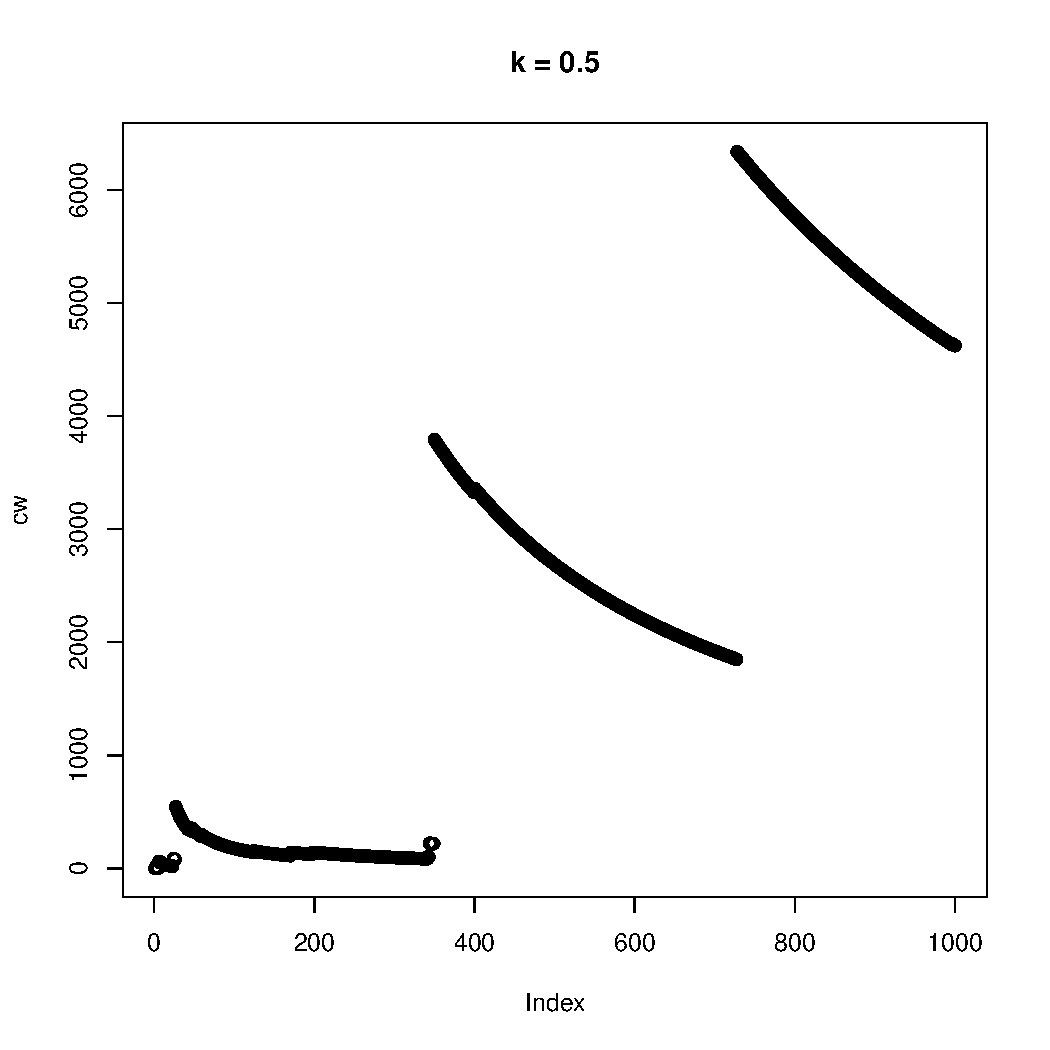
\includegraphics[width=.3\textwidth, page=1]{Rplots.pdf}
	       \includegraphics[width=.3\textwidth, page=2]{Rplots.pdf}
	       \includegraphics[width=.3\textwidth, page=3]{Rplots.pdf}
           \caption{Breiten der Konfidenzintervalle}
       \end{figure}
       Anmerkung: Die $x$-Achse repräsentiert Anzahl der ersten n
       berücksichtigten Samples mit $2\leq n \leq 1000$, die $y$-Achse
       repräsentiert die Breite der Konfidenzintervalle. Die konkrete
       Darstellung ist stark von der zufälligen Eingabe abhängig.

       \newpage
       \lstinputlisting{aufgabe-12.1.R}


    \item %.2
        \begin{enumerate}
            \item
                Die Inversionsmethode kann angewendet werden, da die
                Verteilungsfunktion explizit vorliegt.
                \begin{equation*}
                    F(x) =
                    \begin{cases}
                        0          , & x < 1        \\
                        \frac{1}{6}, & 1 \leq x < 2 \\
                        \frac{2}{6}, & 2 \leq x < 3 \\
                        \frac{3}{6}, & 3 \leq x < 4 \\
                        \frac{4}{6}, & 4 \leq x < 5 \\
                        \frac{5}{6}, & 5 \leq x < 6 \\
                        1          , & 6 \leq x     \\
                    \end{cases}
                \end{equation*}
                Auch die Pseudoinverse $F^{-1}$ kann explizit angegeben werden.
                \begin{equation*}
                    F^{-1}\colon (0,1) \to \mathbb{R}
                    \qquad
                    F^{-1} =
                    \begin{cases}
                        1,  & y \leq \frac{1}{6}               \\
                        2,  & \frac{1}{6} < y \leq \frac{2}{6} \\
                        3,  & \frac{2}{6} < y \leq \frac{3}{6} \\
                        4,  & \frac{3}{6} < y \leq \frac{4}{6} \\
                        5,  & \frac{4}{6} < y \leq \frac{5}{6} \\
                        6,  & \frac{5}{6} < y                  \\
                    \end{cases}
                \end{equation*}

            \item
                Die ersten fünf Werte gemäß der Inversionsmethode sind in der
                folgenden Tabelle aufgetragen.
                \begin{table}[H]
                    \centering
                    \begin{tabular}{c|l|l|l|l|l}
                        $i$   & 1 & 2 & 3 & 4 & 5 \\ \hline
                        $u_i$ & \num{0.1} & \num{0.32} & \num{0.88} & \num{0.02} & \num{0.7} \\ \hline
                        $x_i$ & 1 & 2 & 6 & 1 & 5 \\
                    \end{tabular}
                \end{table}

            \item
                Sei $p_k = \prob(X_1 = k)$ die reale und $p_k^{(0)} = \prob(X_1
                = k) = \frac{1}{6}$ die gewünschte Wahrscheinlichkeit für $k
                \in \{1, \dotsc, 6\}$.
                Da wir die Behauptung unserer Kollegin belegen wollen, testen
                wir $H_0\colon p_k = p_k^{(0)}$ gegen $H_1\colon p_k \neq
                p_k^{(0)}$.
                Dazu verwenden wir den $\chi^2$-Test.
                \lstinputlisting{aufgabe-12.2.R}
                \lstinputlisting{aufgabe-12.2.Rout}
                Da der berechnete $p$-Wert \num{0.01363} kleiner als $\alpha =
                \num{0,05}$. Daher wird $H_0$ abgelehnt und die Aussage der
                Kollegin auf einem Signifikanzniveau von \num{0,05} belegt.
                Wir gehen daher davon aus, dass die gelieferten Zufallszahlen
                $u_1, \dotsc, u_{720}$ nicht auf $[0,1)$ gleichverteilt sind.

        \end{enumerate}

    \item %.3
        Es seien die Dichten $f_X$ und $f_Z$ wie folgt gegeben.
        \begin{equation*}
            f_X(x) =
            \begin{cases}
                \frac{3}{4} (1-x^2), & |x| \leq 1 \\
                0,                   & |x| > 1    \\
            \end{cases}
            \qquad\qquad
            f_Z(x) =
            \begin{cases}
                1 - |x|, & |x| \leq 1 \\
                0,       & |x| > 1    \\
            \end{cases}
        \end{equation*}
        Weiterhin steht eine Möglichkeit zur Generierung von uniform verteilten
        Zufallszahlen auf $[0,1)$ zur Verfügung.
        \begin{enumerate}
            \item
                Die Dichten $f_X$ und $f_Z$ werden durch $g_X$ und $g_Z$ nach
                oben beschränkt:
                \begin{equation*}
                    f_X(x)
                    \leq g_X(x)
                    = \frac{3}{2} \cdot f_Y(x)
                    \qquad\qquad
                    f_Z(x)
                    \leq g_Z(x)
                    = 2 \cdot f_Y(x)
                \end{equation*}
                Der Faktor $c$ wird hier so gewählt, dass die Dichte $f_Y$ (im
                Intervall $[-1,1]$ gleich $\frac{1}{2}$) auf das Maximum von
                $f_X$ bzw. $f_Z$ scaliert wird. Dieses beträgt $\frac{3}{4}$
                bzw. $1$.

                Dabei sei $f_Y$ die Dichte einer Gleichverteilung auf $[-1,1)$.
                Seien $y'_i$ Zufallszahlen, die gemäß einer Gleichverteilung
                aus $[0,1)$ gezogen wurden. Dann sind $y_i = 2y'_i - 1$
                gleichverteilte Zufallszahlen aus $[-1,1)$.

                Um mit der Acceptance-Rejection-Methode Zufallszahlen gemäß der
                Dichte $f_X$ bzw. $f_Z$ zu erzeugen, wird wie folgt vorgegangen:
                \begin{enumerate}
                    \item
                        Generiere eine Zufallszahl $y$ gemäß $f_Y$.

                    \item
                        Generiere eine Zufallszahl $u$ gemäß einer
                        Gleichverteilung auf $[0,1)$.

                    \item
                        Falls $u \leq \frac{f_X(y)}{g_X(y)}$ bzw. $u \leq
                        \frac{f_Z(y)}{g_Z(y)}$ gebe $y$ zurück, sonst beginne
                        wieder mit Schritt i.

                \end{enumerate}
                Die zurückgegebene Zahl $y$ ist gemäßt $f_X$ bzw. $f_Y$
                verteilt.

            \item
                Für $c \to \infty$ gilt $\frac{f_X(y)}{g_X(y)} =
                \frac{f_X(y)}{c \cdot f_Y(y)} \to 0$. Je größer $c$ ist, desto
                kleiner ist also der Bereich, in dem die Zufallszahl abgelehnt
                wird. Man sollte $c$ also möglichst klein wählen, um weniger
                Zufallszahlen zu verschwenden.

            \item
                Würden die gleichen Zufallszahlen zum Erzeugen einer
                Realisierung von $X_{2n-1}$ und $Z_{2n}$ verwendet werden, so
                wären $X_{2n-1}$ und $Z_{2n}$ nicht länger stochastisch
                voneinander unabhängig.

        \end{enumerate}

\end{enumerate}

\end{document}

